\documentclass[a4paper,11pt,oneside,openany]{jsbook}
\usepackage{myjlabthesisstyle}
\daigaku{青山学院大学}
\gakubu{社会情報学部}
\gakka{社会情報学科}
\syubetsu{卒業論文}
\labname{宮治研究室}
\chiefexaminer{宮治~~裕~~教授}

%%%%%%%%%%%%%%%%%%%%%%%%%%%%%%%%%%%%%%%
% ここから先「ここまで個人設定」の範囲に
% 各自の固有の情報を記入して下さい
%%%%%%%%%%%%%%%%%%%%%%%%%%%%%%%%%%%%%%%
\nendo{2021年度}
\teisyutsu{2022年~~1月}
\snum{18118047}
\jname{黒川~~皇輝}
\thesistitle{PLSAとMAP推定を用いた日本語歌詞の印象推定手法の評価} %タイトルを記入
%\thesissubtitle{\LaTeX の利用} %サブタイトルを記入 ない場合はコメントアウト
%\SUBTtrue %サブタイトル有りの場合 ない場合は,コメントアウト
\SUBTfalse %サブタイトル無しの場合 有る場合は,コメントアウト
%%%%%%%%%% ここまで個人設定 %%%%%%%%%%%%%%
\begin{document}

\chapter{システム構成図の例}
システム構成図が論理的に描けると、論文そのものの説明もしやすくなる。
ここでは、シスム構成図の例をいくつか記載する。
\begin{figure}[h]
  \centering
  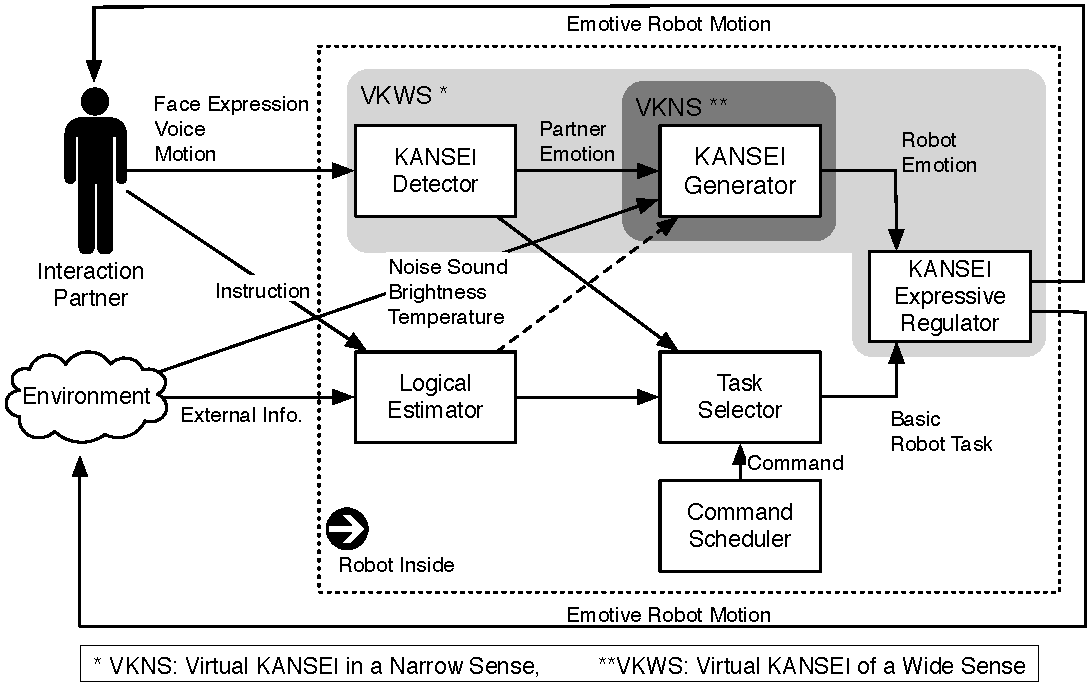
\includegraphics[width=12cm]{VKall.pdf}
  \vspace{-1mm}
  \caption{擬似感性の構成}
  \label{fig:vkall}
  \vspace{5mm}
\end{figure}

\begin{figure}[h]
  \centering
  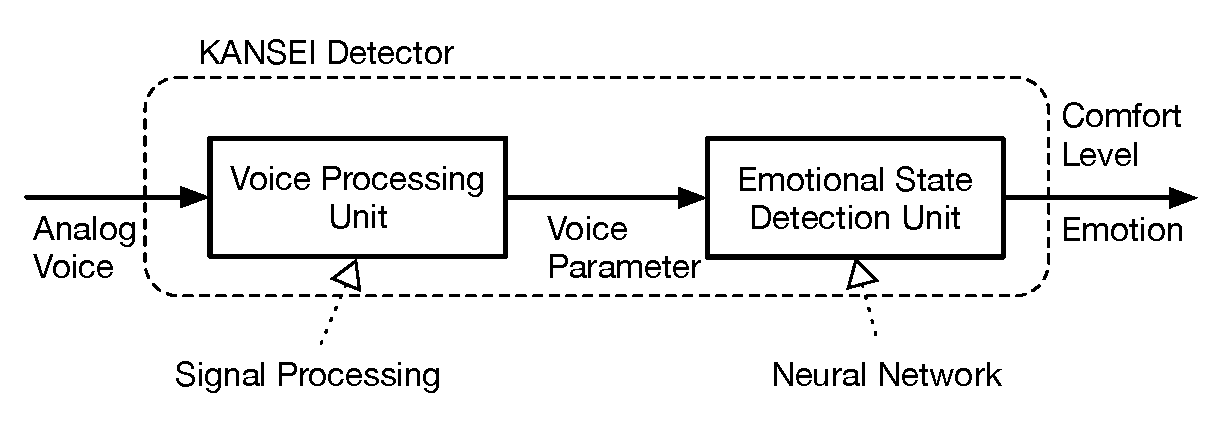
\includegraphics[width=14cm]{VoiceKANSEIDetector.pdf}
  \vspace{-1mm}
  \caption{音声からの感性同定部}
  \label{fig:VoiceKANSEIDetector}
  \vspace{5mm}
\end{figure}
% \begin{figure}[bt]
%     \centering
%     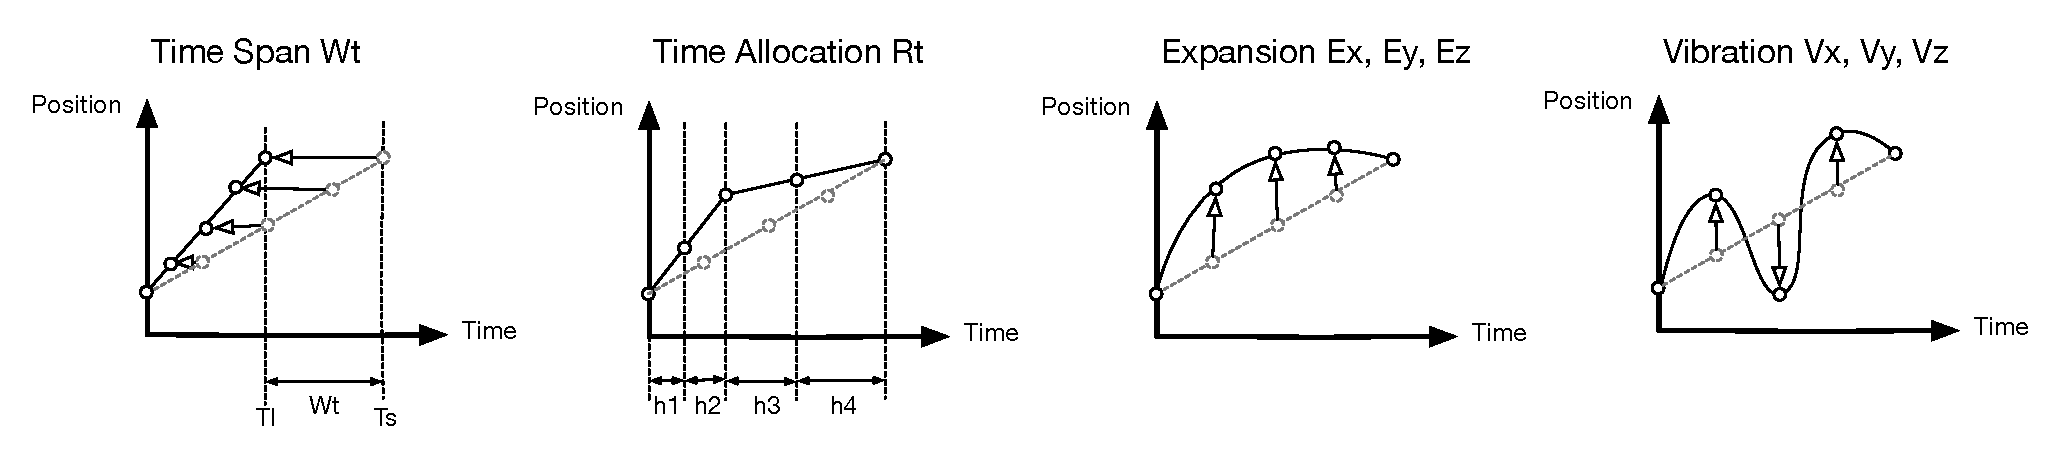
\includegraphics[width=14cm]{mp2.pdf}
%     \vspace{-1mm}
%     \caption{MMSの内部構成}
%     \label{fig:mp2}
%     \vspace{5mm}
% \end{figure}
%
\end{document}